\documentclass[a4paper,10pt,headlines=3.2]{scrartcl}

%Für Windows:
%\usepackage[T1]{fontenc}		%Umlaute
%\usepackage[latin1]{inputenc}		%latin-Zeichensatz

%\usepackage[colorlinks]{hyperref}	%Hyperlinks + Verlinkung innerhalb von PDFs

\usepackage{ucs}			%Formatierung (Linux)
\usepackage[utf8]{inputenc} 		%Umlaute Linux
\usepackage{graphicx}           	%Bilder
\usepackage[ngerman]{babel}		%Deutsche Sprache
\usepackage{amsmath}			%Math. Zeichen
\usepackage{pifont}			%Skalierbare Schriftart
\usepackage{array}			%Arrays
\usepackage{epsfig}			%Erweiterte Grafiken
\usepackage{makeidx}			%Stichwortverzeichnis
\usepackage[pdftex]{color} 		%Farbige PDFs
\newcommand{\changefont}[3]{    	%Definition von Schriftarten
\fontfamily{#1} \fontseries{#2} \fontshape{#3} \selectfont}
\makeindex				%Inhaltsverzeichnis erstellen
\usepackage[automark]{scrpage2}		%scrpage
%\usepackage[nosectionbib]{apacite}	%Zitieren nach APA
\usepackage{lmodern}			%Font: Latin modern
\usepackage{scrpage2}           	%KOMA-Script
\usepackage{tipa}			%Phonologische Symbole
%\usepackage{qtree}			%Baumstrukturen
\usepackage{pgf}			%Rastergrafiken
\usepackage{remreset}			%Fussnoten global
\usepackage{pdfpages}
\makeatletter				
\@removefromreset{footnote}{chapter}	
\makeatother 				
\setcounter{tocdepth}{3}		%Inhaltsverzeichnis bis auf Tiefe 3 ausgeben
\pagestyle{scrheadings}         	%Kopfzeilen: Seitenstil scrheadings verwenden
\changefont{cmss}{m}{n}			%Schriftart: Computer-Schrift
\usepackage{listings}			%Java-Quellcode ausgeben
\lstset{numbers=left, numberstyle=\tiny, numbersep=5pt} \lstset{language=Java} 


%Manuelle Einstellung der Seitengrösse. Sonst automatisch, siehe unten.
%\setlength{\textheight}{24cm}
%\setlength{\textwidth}{16cm}
%\setlength{\topmargin}{-2cm}
%\setlength{\oddsidemargin}{0cm}

% Groesse des Textbereiches in der Seite
\setlength{\textwidth}{16cm}
\setlength{\textheight}{22cm}
% Kopf- und Fusszeile, Hoehe und Abstand vom Text
\setlength{\headheight}{15pt}
\setlength{\headsep}{0.8cm}

%----------- wird automatisch berechnet
% Linker Seiteneinzug
\setlength{\oddsidemargin}{2.5cm} \addtolength{\oddsidemargin}{-1in}
\setlength{\evensidemargin}{2.5cm} \addtolength{\evensidemargin}{-1in}
% Andere Groessen ausrechnen (vertikal zentrieren)
\setlength{\footskip}{\headsep}
\addtolength{\footskip}{\headheight}
\setlength{\topmargin}{\paperheight}
\addtolength{\topmargin}{-\textheight}
\addtolength{\topmargin}{-\headheight}
\addtolength{\topmargin}{-\headsep}
\addtolength{\topmargin}{-\footskip}
\addtolength{\topmargin}{-2in}
\addtolength{\topmargin}{-0.5\topmargin}
%----------- 

\setlength{\headheight}{20pt}		%Abstand zurücksetzen für Kopfzeile (3 Zeilen)
\setheadsepline{.4pt}			%Separate Linie im Kopf
\clearscrheadfoot
\ihead[]{Einführung in die Informatik \\Herbstsemester 2011 \\Institut für angew. Math. und Informatik} % - links
\ohead[asdasd]{Übung 1, 14. Okt 2011 \\Gino Torriani [06-128-714] \\ Adrianus Kleemans [07-111-693]} % - linke Kopfzeile 
\cfoot[\pagemark]{\pagemark} 		%mittlere Fusszeile 

\newcommand*\f[1] {\textbf{#1}}

\begin{document}
\section{Lösungsbeschreibung}
\begin{enumerate}
\item Es wird die gesamte Population von $66$ Generationen à $100'000$ Personen generiert.
\item Die Verwandschaftsbeziehungen werden festgelegt: Zu jeder beliebigen Person aus Generation $p$ werden zwei Elternteile aus Generation $p-1$ ermittelt. Die Wahrscheinlichkeit für ein Individuum aus $p$, ein bestimmtes Individuum aus $p-1$ als Elternteil zu haben, richtet sich nach der Anzahl Personen, also ist sie pro Wahl\footnote{Es findet insgesamt 2 Mal pro Individuum aus $p$ eine Wahl statt, eine für den Vater, eine für die Mutter.} für ein Mitglied der Generation $p-1$ genau $\frac{1}{100000}$.
\item Von Generation $p$, beginnend mit $0$, wird von jedem Individuum nach Nachkommen gesucht. Dies beginnt in $p+1$, wobei alle Nachkommen in einer Liste gespeichert werden. Von den resultierenden Personen wird wiederum nach deren Nachkommen gesucht. Dies wiederholt sich bis in die 66. Generation ($p = 65$).
\end{enumerate}

\section{Resultate}
Die Resultate erstaunen. Folgende Kennwerte wurden ermittelt:
\begin{itemize}
 \item Der \f{Median} von Nachkommen pro Person aus Generation $134$.
 \item Der \f{Mittelwert} von Nachkommen pro Person aus Generation $0$ beträgt $132.9$.
 \item Der \f{Höchstwert} lag bei 188 Nachkommen.
 \item Der \f{Mindestwert} lag bei 83 Nachkommen.

\begin{figure}[ht]
\centering
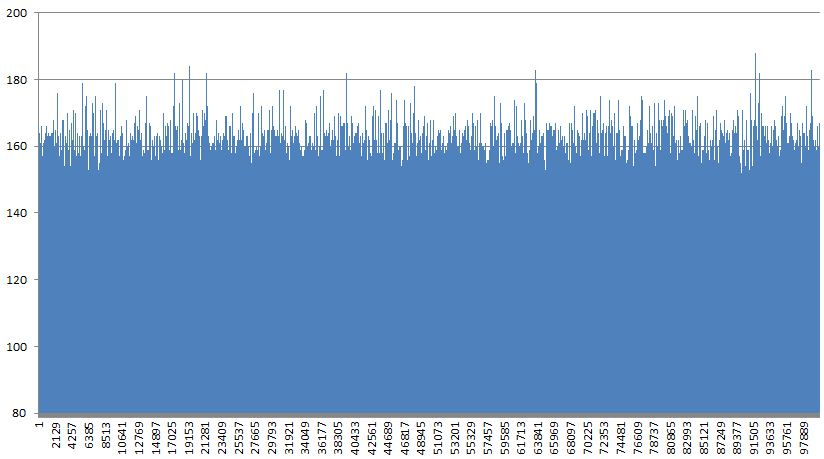
\includegraphics[width=0.9\linewidth]{sample1}
\end{figure}

\end{itemize}
Genauer könnte man die Verteilungsfunktion so beschreiben\footnote{mit der Einschränkung, dass die Berechnung nur auf einer einmaligen Ausführung des Programm beruht}, dass sie eine Normalverteilung mit folgenden Parametern ist:
\begin{itemize}
 \item Standardabweichung $\sigma = 10$
 \item Dichte $\mu = 133$
\end{itemize}

\begin{figure}[ht]
\centering
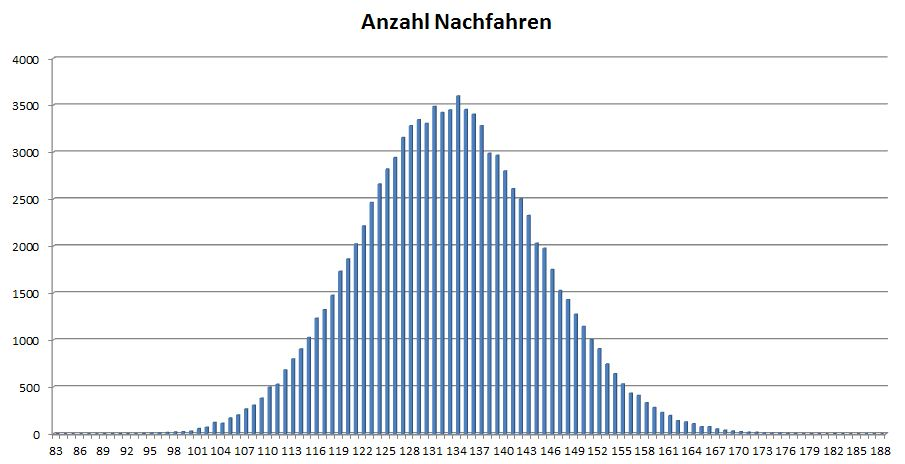
\includegraphics[width=0.9\linewidth]{sample2}
\end{figure}

\subsection{Spezialfall: Keine Nachkommen}
Für den Fall, dass jemand keine Nachkommen haben sollte, lässt sich die Wahrscheinlichkeit berechnen:

\begin{eqnarray}
p = \frac{e^{\frac{-1}{200} (-133)^2}}{10 \sqrt{2 \pi}} \\
\Rightarrow p = \frac{1}{10 e^{\frac{17689}{200}} \sqrt{2\pi}}\\
p\approx 1.54787\cdot 10^{-40} \\
\approx 1 : 6'460'000'000'000'000'000'000'000'000'000'000'000'000
\end{eqnarray}

Es ist also extrem unwahrscheinlich, dass jemand keine/n oder nur eine/n\footnote{1 Nachfahre: $p \approx 5.82337\cdot 10^{-40}$} Nachfahren hat.

\section{Anhang: Java-Klassen}
Im Anhang finden sich 3 Java-Klassen:
\begin{itemize}
 \item \f{Main.java} - Das ausführbare Hauptprogramm, inkl. Tracing\footnote{Zur Funktionsweise: Siehe Funktion \textit{trace()}}-Algorithmus.
 \item \f{Generation.java} - repräsentiert eine Generation, welche mit Personen ``bevölkert'' wird.
 \item \f{Person.java} - repräsentiert eine Person mit festgelegten Attributen für die Elternteile. 
\end{itemize}

%PDF einbinden
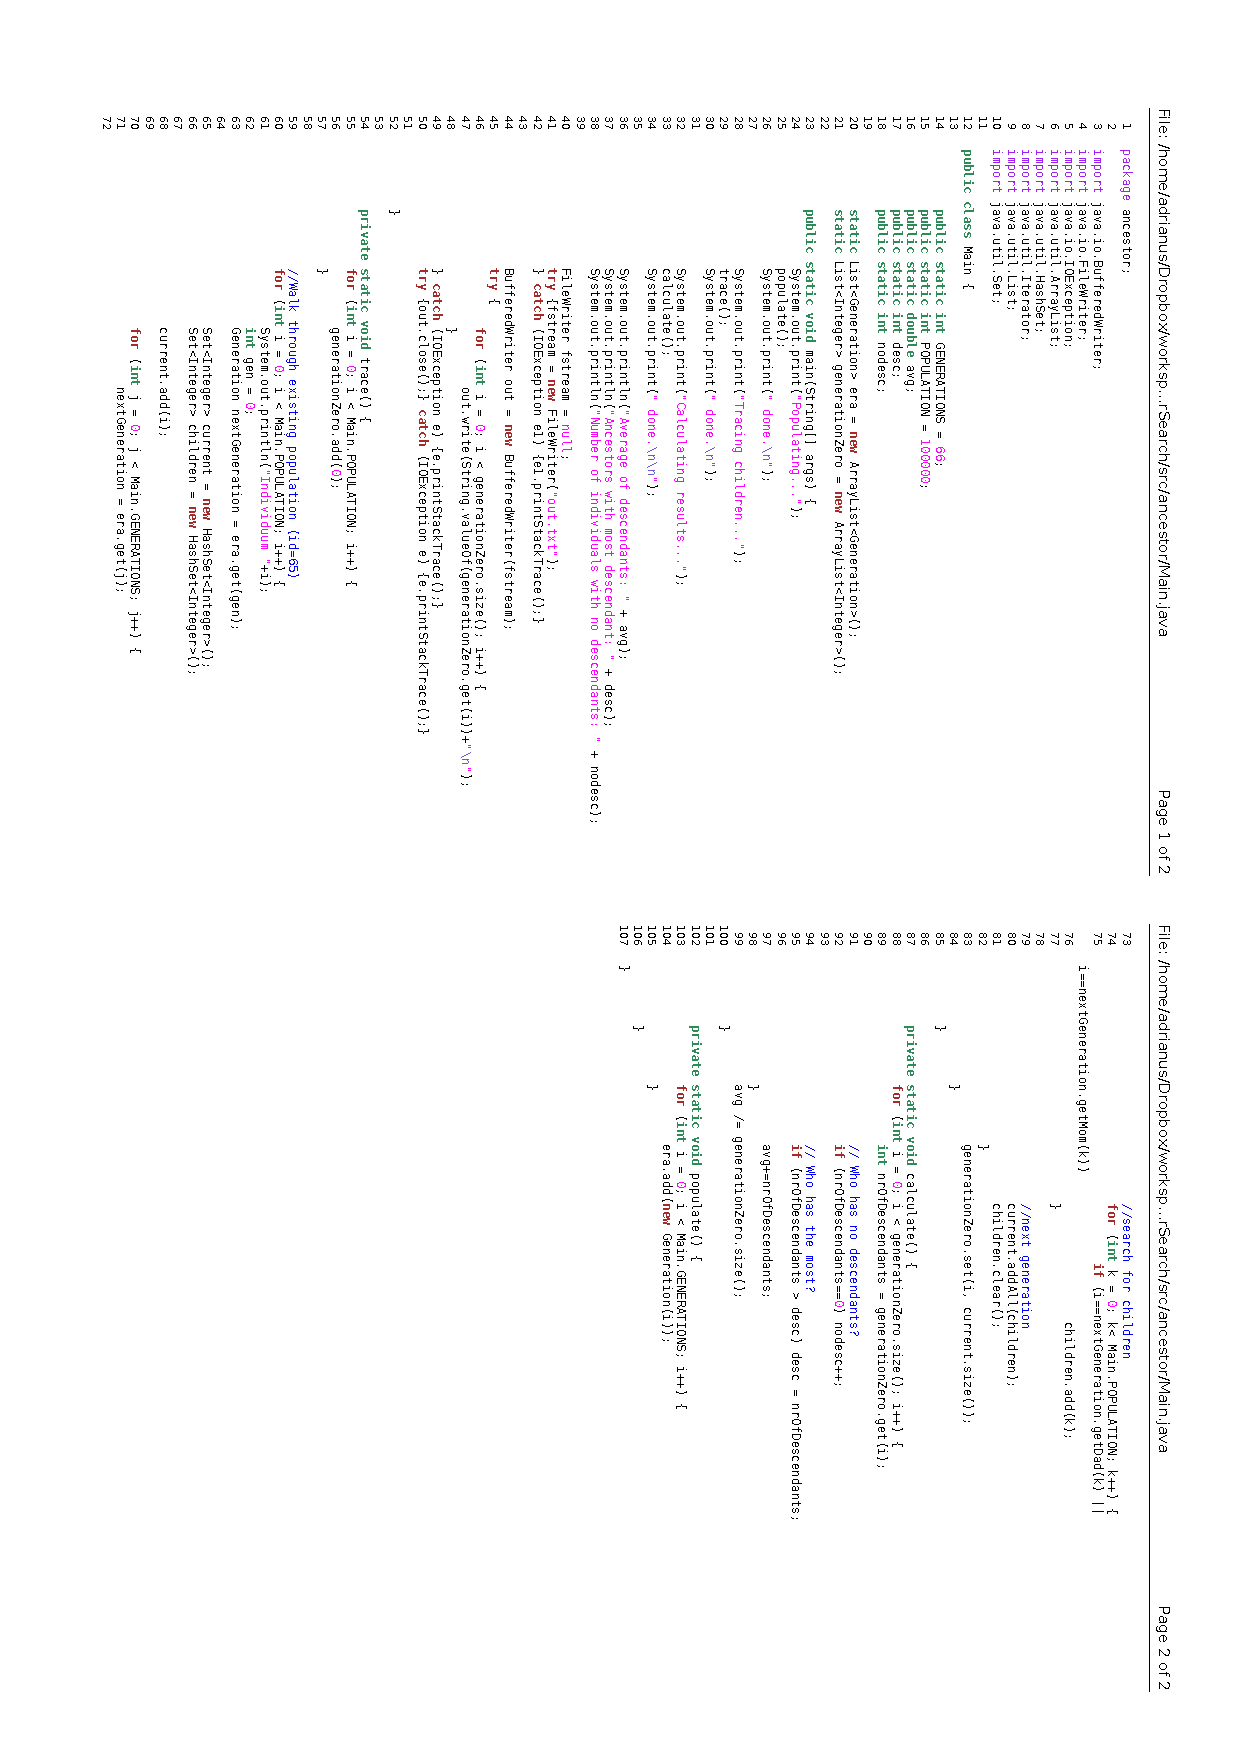
\includepdf{main.pdf}
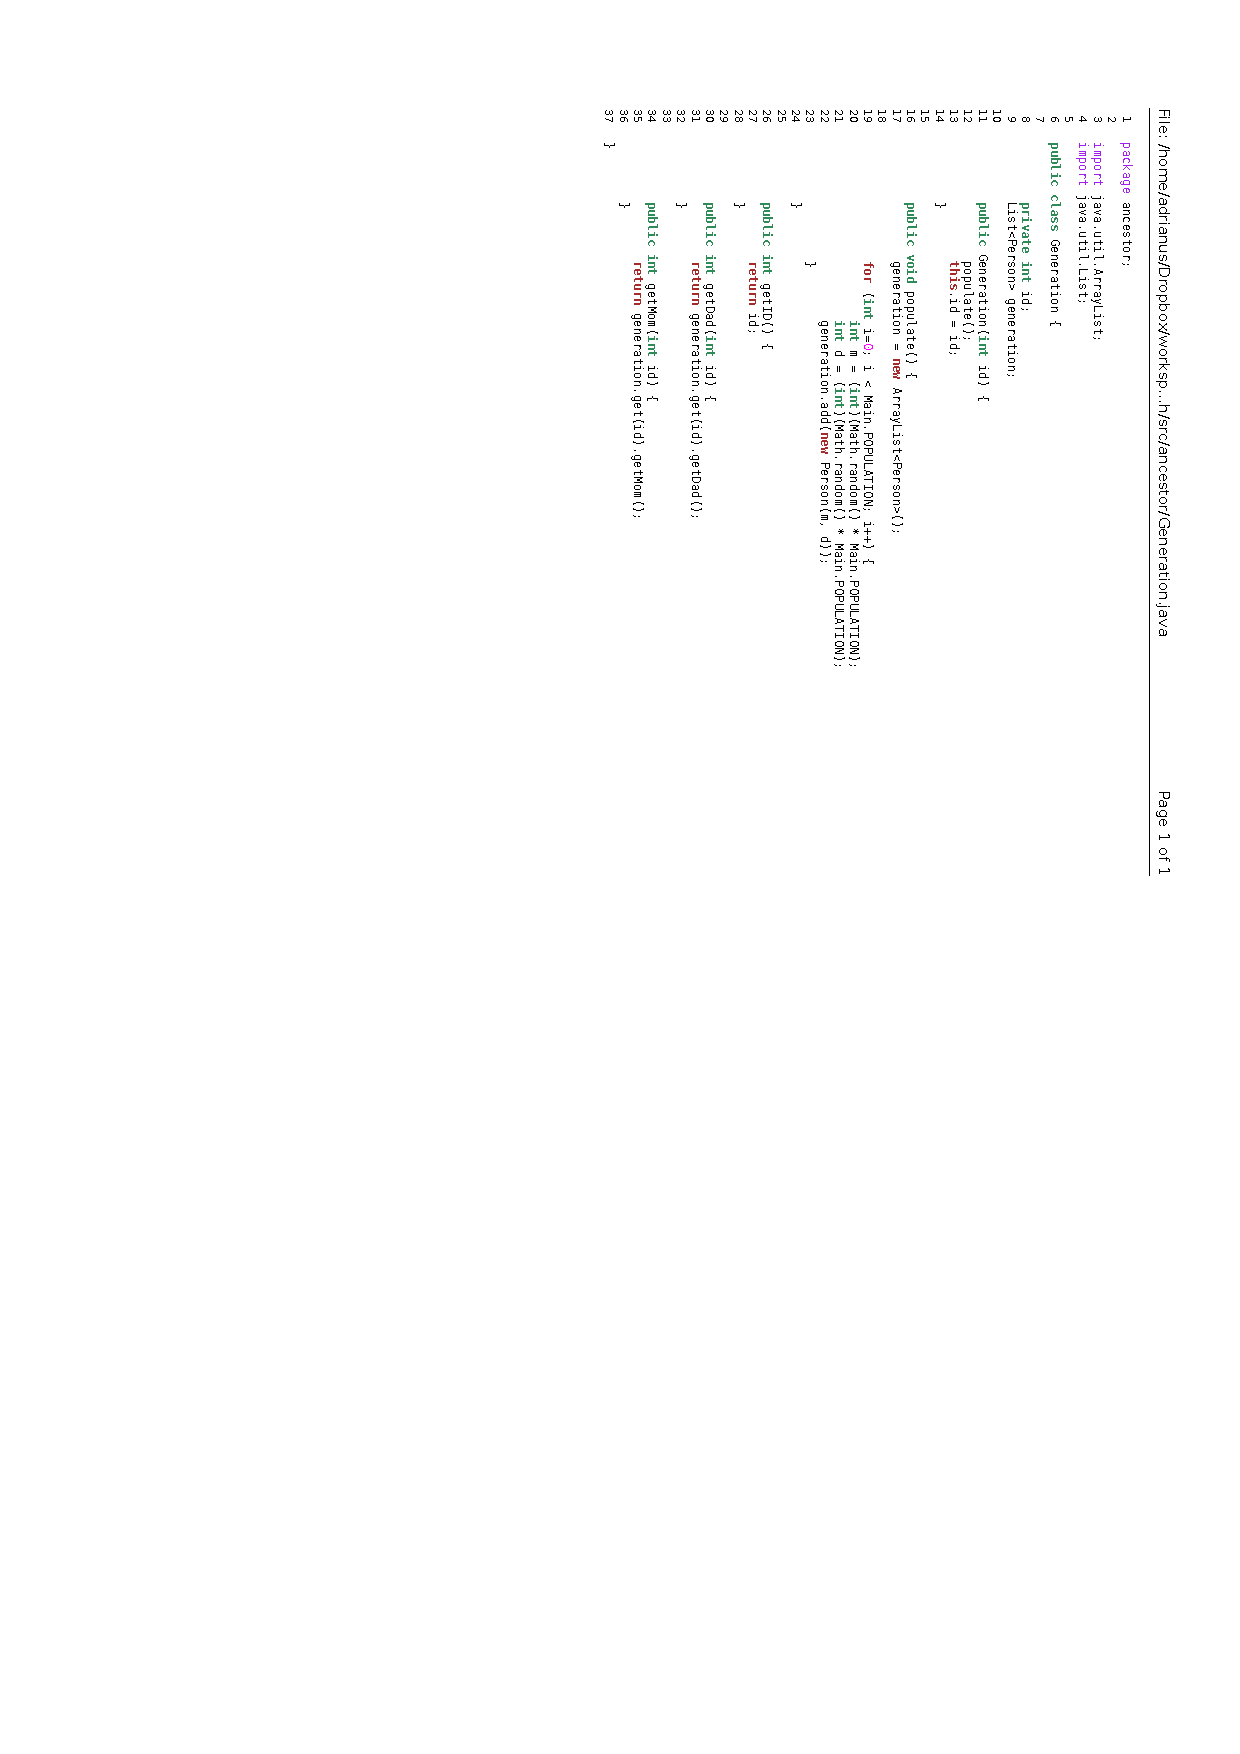
\includepdf{generation.pdf}
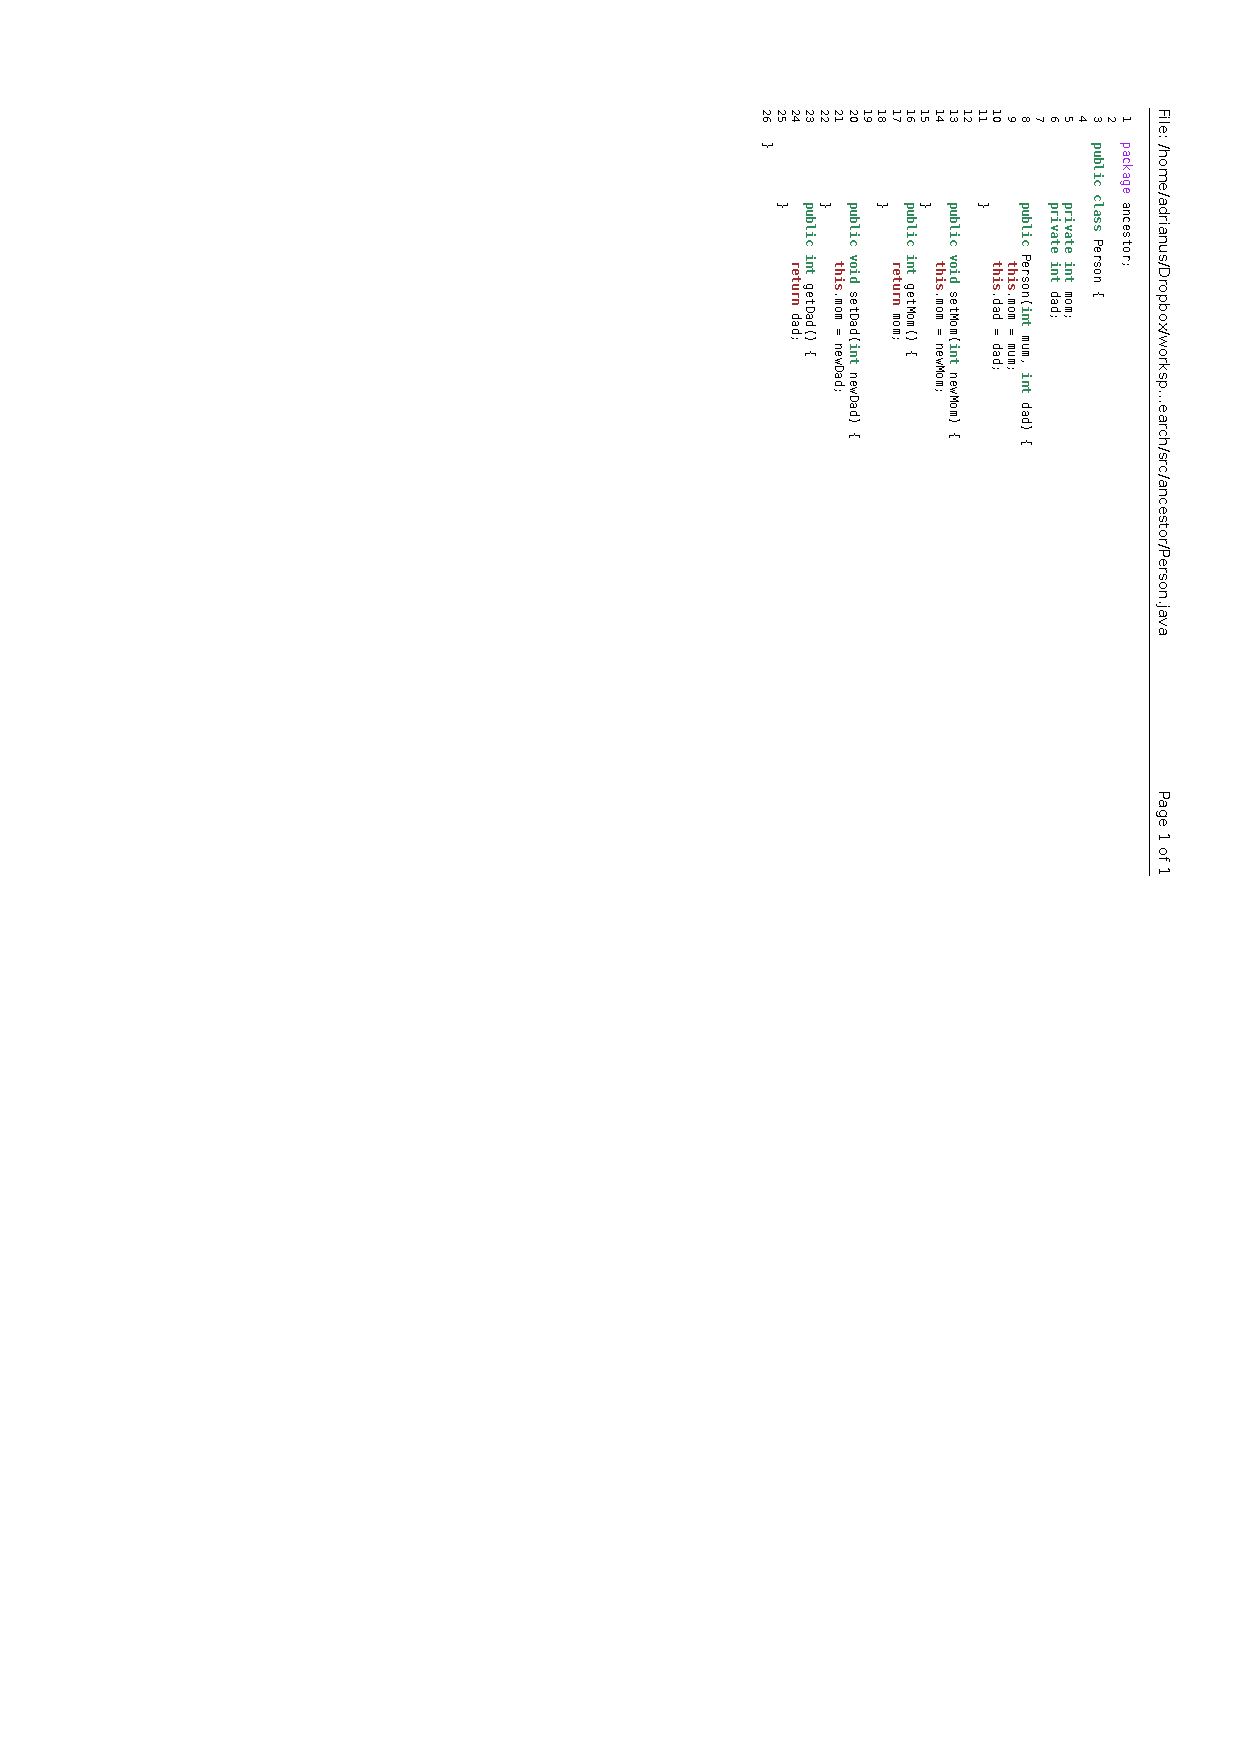
\includepdf{person.pdf}

\end{document}
